\chapter{Introdução}
\label{intro}

Em Portugal a percentagem da população idosa (65 anos ou mais) tem vindo a aumentar gradualmente nos últimos 60 anos. Este facto, juntamente, com o aumento do índice de dependência idosa e a alteração da estrutura familiar predominante no ultimo século em Portugal, veio trazer à luz do dia a problemática do acompanhamento dos idosos que vivem sozinhos, ou que requerem vigilância regular.
Esta é uma questão que já foi reconhecida por outros países, onde existem serviços já desenvolvidos e implementados com o objectivo de melhorar a qualidade de vida destes idosos. Chegando ao ponto de se tornar numa industria de serviços com muita procura e oferta diversificada. Em Portugal este é um nicho de mercado ainda pouco explorado, onde existe pouca oferta e com muito pouca inovação ou desenvolvimento.
Foi com estas informações em mente que nos foi proposto, no âmbito da disciplina de Projecto Integrado, que desenvolvesse-mos a análise, desenho e implementação de um sistema de tele-assistência por dispositivo móvel. Sempre com objectivo de tentar assegurar a autonomia e qualidade de vida do utente, através da detecção de emergências em tempo real, facilitando assim a comunicação e assistência para  com o utente do serviço.
A nossa principal preocupação prendeu-se com a portabilidade e capacidade de utilização do sistema em ambientes exteriores ao domicilio, tendo para isso criado um prototipo portátil, sem ligações físicas de energia ou comunicações, permitindo assim uma total mobilidade do utente.
Analisamos alguns dos dispositivos presentes nos mercados dos estados Unidos da América, Reino Unido e Austrália, pois este foram os países que apresentaram uma maior oferta de serviços.
Este dispositivo foi criado com base num arduino, adicionando diversos módulos que nos garantiram as funcionalidade pretendidas.

%Duas citações \cite{book:Brooks1995,Chen1976}.

\section{Análise do estado da arte}

O mercado dos serviços na 3ª idade tem-se vindo a desenvolver bastante, tendo surgido diversos sistemas e serviços que possuem como finalidade facilitar e melhorar a vida dos idosos. Os principais mercados mundiais situam-se nos EUA e na Grã-Bretanha, onde este tipo de sistemas e serviços abundam. Foi essencialmente nesses mercados que encontramos sistemas semelhantes, os quais analisamos de modo a determinar quais são as características que deveríamos incluir no nosso protótipo.
Os sistemas apresentados dividem-se basicamente em wereables (sistemas que se utilizam pendurados ou em contacto com o corpo do utilizador) e os fixos (caixas que estão estáticas numa localização da residência).
Os wearebles possuem sensores que permitem detectar quedas, no entanto pelo que apuramos reportam um elevado número de falsos positivos. O grande problema parte da incapacidade de diferenciar entre as origens das acelerações que o sensor regista. Outro problema destes sistemas prende-se com a pequena capacidade das suas baterias, geralmente na ordem dos 900 mAh, o que implica que a sua autonomia é relativamente pequena. O seu tamanho e simplicidade de operação, tornam o sistema bastante portátil, no entanto também causam limitações ao nível da usabilidade, uma vez que o número de acções e facilidade de executar as mesmas torna-se limitada. Por fim à a referenciar a capacidade de ligar-se através de rede 3G para efectuar a transmissão de dados.

As figuras \ref{fig:sistema_portable_1}, \ref{fig:sistema_portable_2} e \ref{fig:sistema_portable_3} apresentam alguns dos dispositivos wearebles analisados.

% O pacote subfigure não consegue colocar as imagens lado a lado
\begin{figure}[!htb]
	\centering
	\begin{minipage}[b]{0.3\textwidth}\centering
		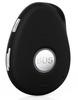
\includegraphics[width=3cm]{figuras/Sistemas_alert_Alarm_Australia.jpg}
		\caption{Elderlly fall button para seniores da Alert Alarm Australia}
		\label{fig:sistema_portable_1}
	\end{minipage}
	\hfill
	\begin{minipage}[b]{0.3\textwidth}\centering
		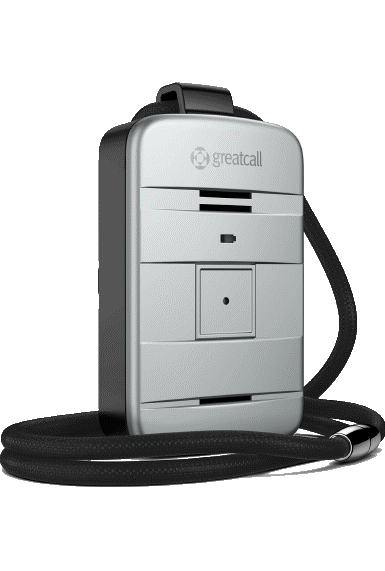
\includegraphics[width=3cm]{figuras/Sistemas_MedicalAlert.png}
		\caption{Mobile elite System da MedicalAlert}
		\label{fig:sistema_portable_2}
	\end{minipage}
	\hfill
	\begin{minipage}[b]{0.3\textwidth}\centering
		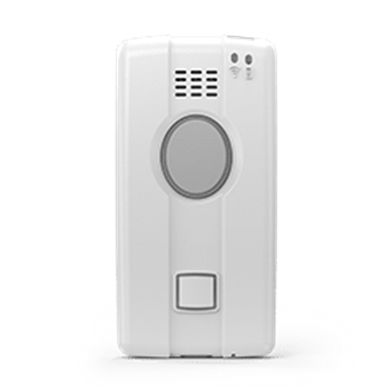
\includegraphics[width=3cm]{figuras/Sistemas_Bluestar.png}
		\caption{Admiral Alert da BlueStar Senior Tech}
		\label{fig:sistema_portable_3}
	\end{minipage}
\end{figure}

A segunda categoria é os sistemas fixos. Este não são tão versáteis, apresentam mais funcionalidades. Alguns modelos permitem a detecção de quedas, mas é necessário um pendente que adiciona essas funções. As suas maiores dimensões permitem que os sistemas possuam sistemas sonoros integrados, o que permite a comunicação com os utilizadores através do sistema de teleassistência. Além disso as maiores dimensões permitem que existam mais possibilidade para adicionar botões e écrans que poderão permitir uma maior usabilidade quando comparado com os wereables. Estes tipos de sistemas, possuem ligações a linhas telefónicas físicas e à energia eléctrica, o que permite que a sua autonomia seja ilimitada.
As figuras \ref{fig:sistema_fixed_1} e \ref{fig:sistema_fixed_2} apresentam alguns dos dispositivos fixos analisados.
\vspace*{-11cm}
\begin{figure}[!htb]
	\centering
	\begin{minipage}[b]{0.45\textwidth}\centering
		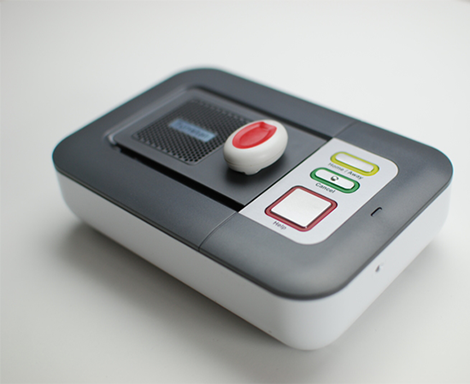
\includegraphics[height=5cm]{figuras/Sistemas_Lifeline.png}
		\caption{Lifeline Vi Alarma Unit da LifelIne24}
		\label{fig:sistema_fixed_1}
	\end{minipage}
	\hfill
	\begin{minipage}[b]{0.45\textwidth}\centering
		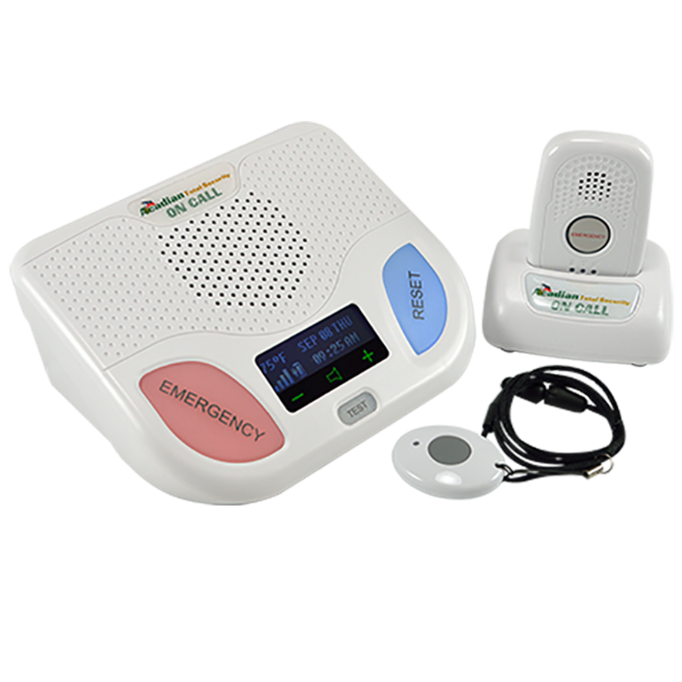
\includegraphics[height=5cm]{figuras/sistemas_Medical_Alert_System.png}
		\caption{Medical Alert System da AcadiaOnCall}
		\label{fig:sistema_fixed_2}
	\end{minipage}
\end{figure}

\pagebreak